\section{Machine réelle}
Nous avons utilisé une machine réelle de récupération équipée d'un processeur Intel Pentium 4 et de 1 Go de RAM. Nous avons décidé de faire celà pour augmenter le challenge et le réalisme du projet. Nous n'avons pas eu beaucoup de problèmes causés par cette machine si ce n'est l'impossibilité d'utiliser LUKS (car la machine manque de puissance) et un problème de carte graphique réglé par le module \texttt{nomodeset} dans Grub.
Nous avons utilisé le RAID1 pour augmenter la sécurité de nos données, nous avons utilisé deux disques de même capacité, ainsi si l'un des deux disque lache il est possible de récupérer l'intégralité des données.
Avant de charger nos fichiers sur la machie réelle nous avons travaillé sur des machines virtuelles nous permettant simplement de gérer les snapshot et de travailler lorsque nous ne sommes pas proche de la machine.
Nous avons aussi ajouté un mot de passe superviseur sur le BIOS pour empécher les modifications ce qui permettrait d'outrepasser le mot de passe sur GRUB.

\begin{figure}[H]
	\centering
	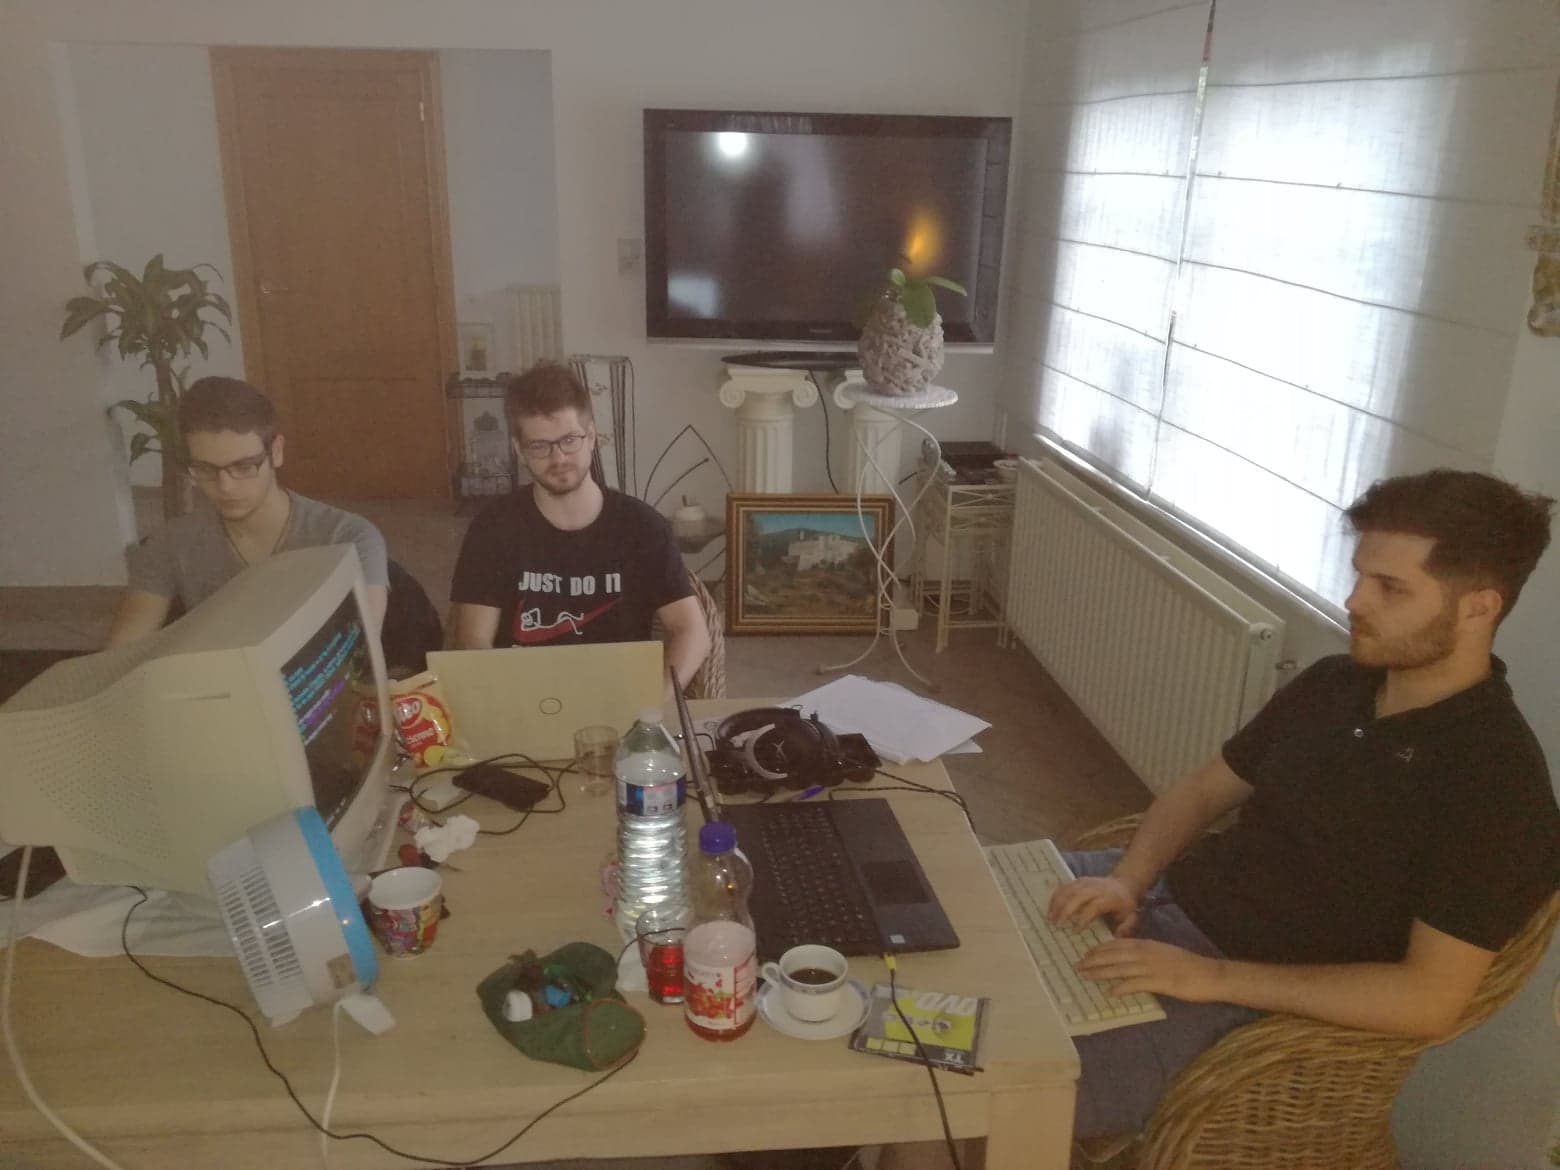
\includegraphics[height=6cm]{textures/images/machineReelle.jpg}
	\caption{\label{fig:machinereelle}Machine réelle}
\end{figure}
